\section{data analysis}
\label{sec:data analysis}

\begin{figure*}
    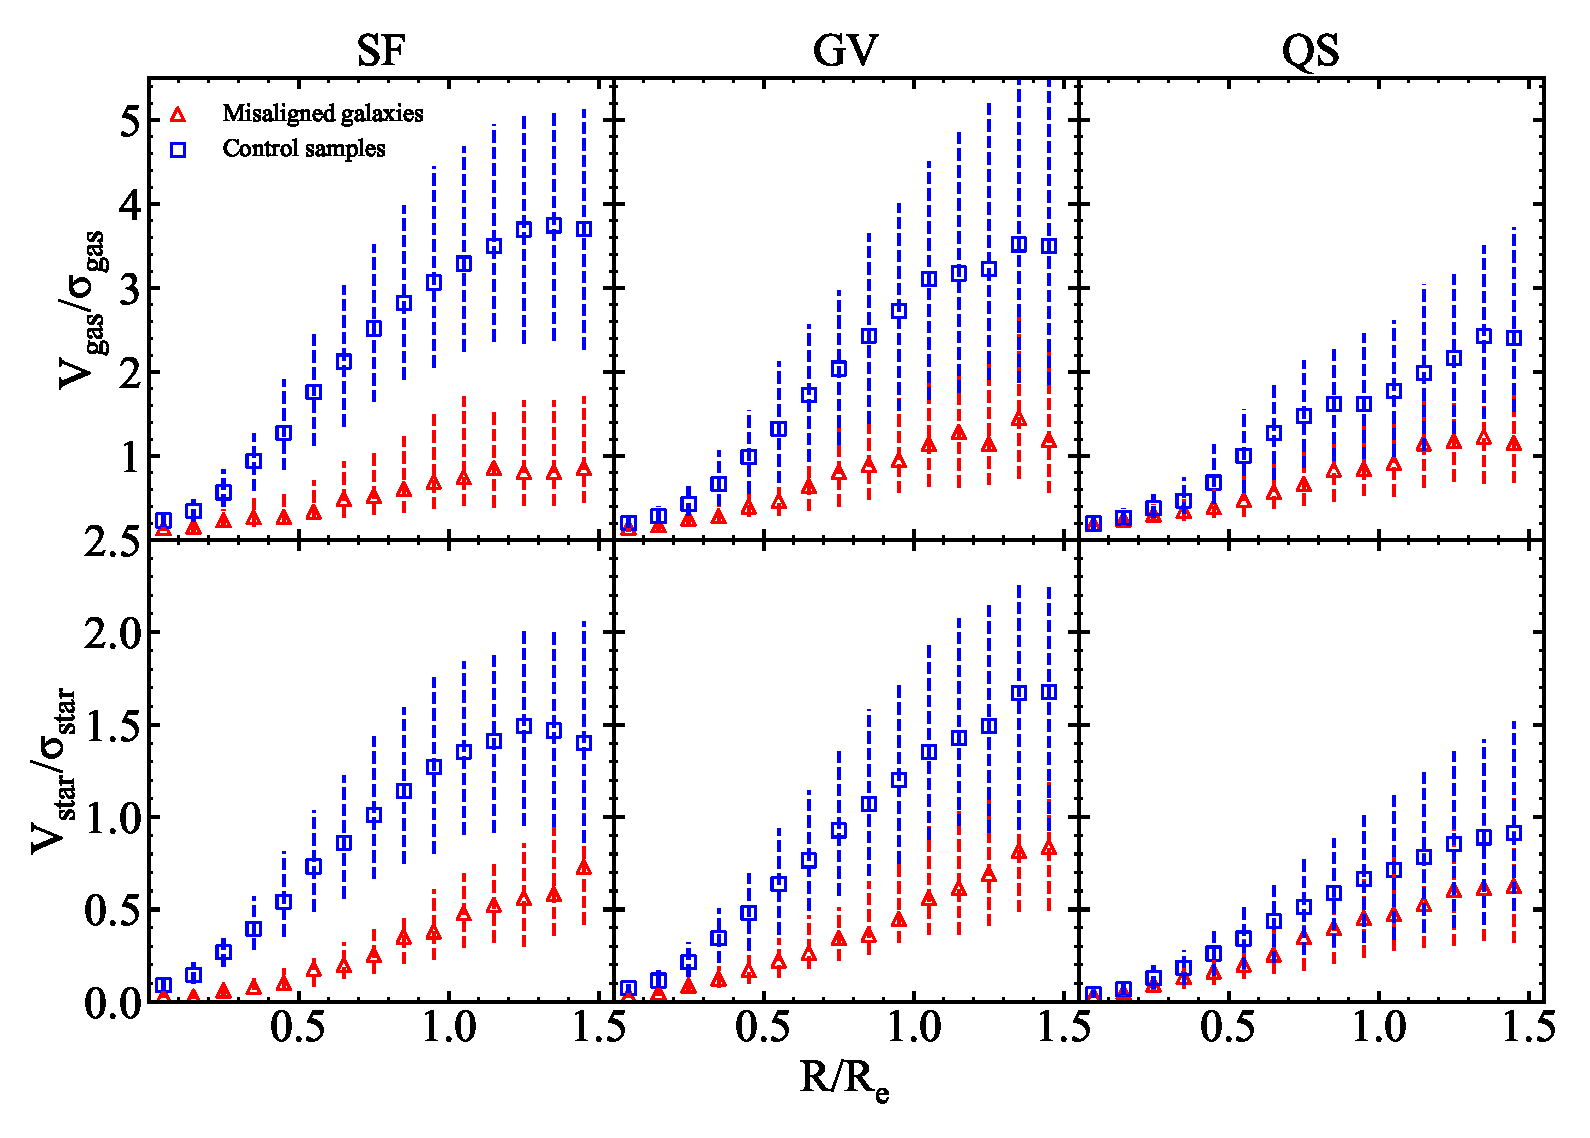
\includegraphics[width=2.0\columnwidth]{pics/vel_divide_sigma_gas_stellar.eps}
    \caption{Comparison of ${\rm V}_{\rm gas}/{\sigma}_{\rm gas}$ (top row) and ${\rm V}_{\rm star}/{\sigma}_{\rm star}$ (bottom row) radial profiles within 1.5 ${\rm R}_{\rm e}$ between misaligned galaxies and control sample. The left panel is for SF, the middle panel is for GV, the right panel is for QS. The red triangles represent the median value of misaligned galaxies and the blue squares represent the median value of control sample. The error bars show the 30th and 70th percentiles of the distribution. The radii are the projected distances from the galactic centre to the spaxels where indices are measured in the unit of the effective radius.}
    \label{fig:vel_divide_sigma}
\end{figure*}

\begin{figure*}
    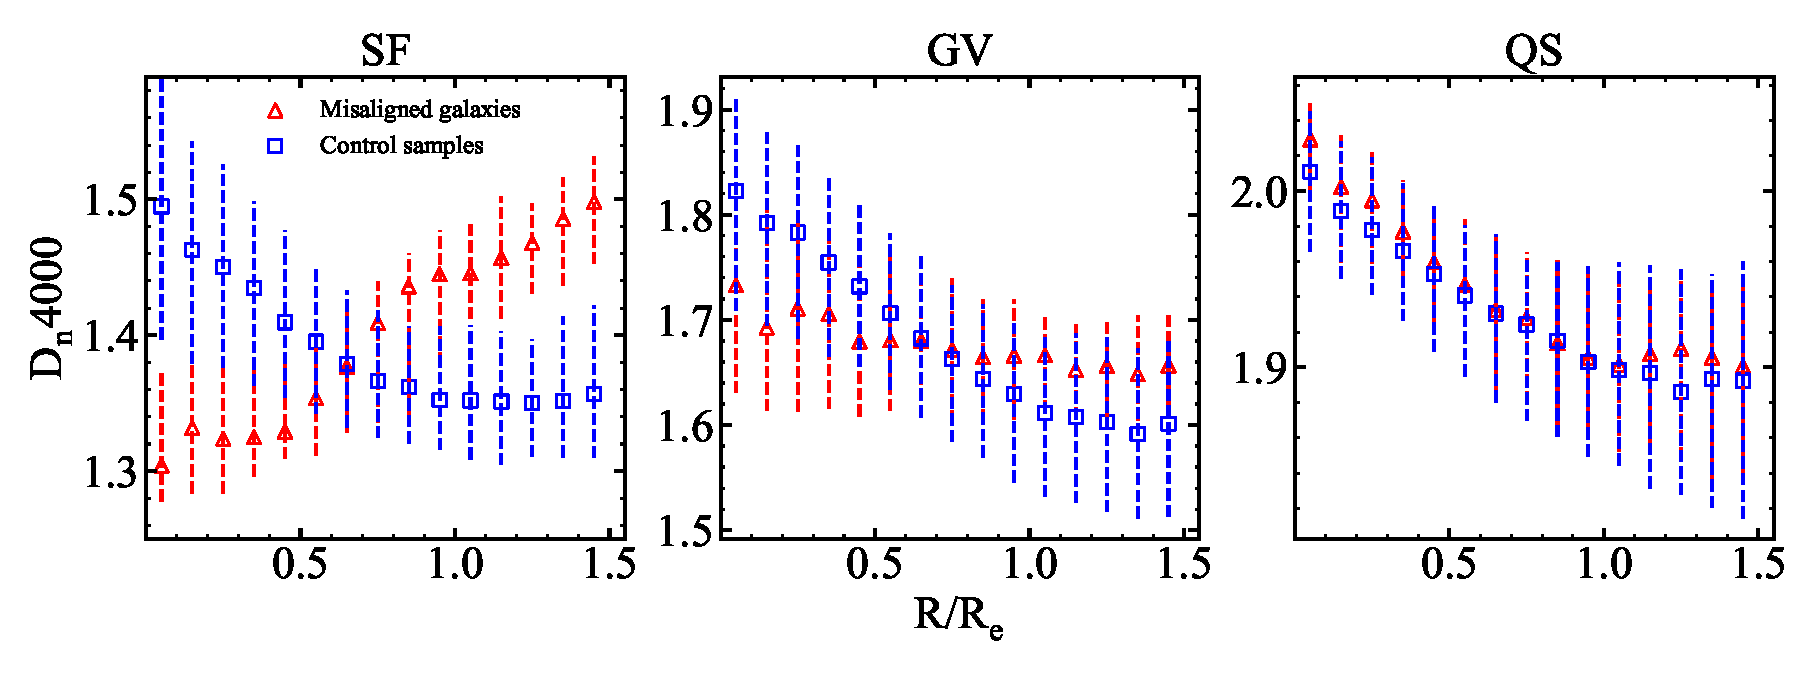
\includegraphics[width=2.0\columnwidth]{pics/Dn_4000.eps}
    \caption{Comparison of D$_n$4000 radial profiles within 1.5 $R_{\rm e}$ between misaligned galaxies and control sample. Red triangles represent misaligned galaxies and blue squares represent control sample.}
    \label{fig:Dn(4000)}
\end{figure*}

In this section, we compare the spatial resolved properties between the misaligned galaxies and their control sample, including the average gas and stellar velocity to velocity dispersion ratio ($V_{\rm gas}/{\sigma}_{\rm gas}$ and $V_{\rm star}/{\sigma}_{\rm star}$), stellar population (D$_n$4000, light and mass-weighted stellar age, on going star forming rate), gas-phase metallicity. We hope to have a picture about the evolution of the misaligned galaxies through this section.

\subsection{Kinematics}

The ratio between ordered to random stellar motion in galaxies is strongly depending on luminosity and stellar mass \citep{veale_massive_2017, green_sami_2018}, which indicates a link between the build-up of stellar mass and angular momentum over cosmic time, which is fundamental in understanding the large variations in morphology and star formation in present-day galaxies. Major mergers are primary candidates for a dramatic changing in the morphology and spin of galaxies, however merger is only one of the many physical processes at play over the lifetime of a galaxy, continuing gas accretion and star formation can reshape the morphology and kinematics of remnants \citep{naab_atlas3d_2014}. In this section, we compare the ratio of radial gradients of velocity to velocity dispersion of gas and stellar components, $V_{\rm gas}/{\sigma}_{\rm gas}$ and $V_{\rm star}/{\sigma}_{\rm star}$, try to discern any difference in the formation/interaction history of the misaligned and control sample.

Fig.~\ref{fig:vel_divide_sigma} shows the median velocity to velocity dispersion ratio for gas and stellar components, $V_{\rm gas}/{\sigma}_{\rm gas}$ (top row) and $V_{\rm star}/{\sigma}_{\rm star}$ (bottom row), along their kinematic major axis for the misaligned sample and the control sample. In each row, the left panel is for SF, the middle panel is for GV and the right panel is for QS. The red triangles represent the median value of the misaligned sample and the blue squares represent the median value of the control sample. The error bars show the 30th and 70th percentiles of the distribution. The larger (smaller) value of $V/\sigma$ corresponds to more (less) rotationally support for the relevant components. $V$/$\sigma$ are taken from MaNGA DAP files, they are estimated from the spectral fitting process described in Sec.~\ref{sec:Sample of kinematically misaligned galaxies}. We can find that SF, GV, QS misaligned galaxies have $V_{\rm gas}/{\sigma}_{\rm gas}$ and $V_{\rm star}/{\sigma}_{\rm star}$ smaller and systematically shifted than their control samples. The difference between misaligned galaxies and control samples in QS is much smaller than that in SF and GV, indicating that external gas accretion has larger influence on the evolution (morphology) of SF, GV galaxies than QS galaxies.

\citet{chen_growth_2016} and \citet{jin_sdss-iv_2016} find that the central regions of star-forming misaligned galaxies show more intense, ongoing star formation and younger stellar populations than their outskirts, suggesting these galaxies accrete abundant external gas, the interaction between accreted and pre-existing gas triggers gas into central regions and forms new stars. The lower value of $V_{\rm star}/{\sigma}_{\rm star}$ and $V_{\rm gas}/{\sigma}_{\rm gas}$ in the star-forming misaligned galaxies than their controls can be easily understood under this picture in the following way: the interaction between accreted external gas and pre-existing gas (in the extreme case, they are counter-rotating) leads to the cancellation of angular momentum, thus lowers $V_{\rm gas}/{\sigma}_{\rm gas}$ as well as $V_{\rm star}/{\sigma}_{\rm star}$ once the gas transforms into stars. 

The GV and QS misaligned galaxies appear to have been undergoing a similar process to that seen in the star-forming misaligned galaxies which lead to the lower value of $V_{\rm star}/{\sigma}_{\rm star}$ and $V_{\rm gas}/{\sigma}_{\rm gas}$ than the control sample, but, on the one hand, the gas accretion and trigger of star formation happened earlier; on the other hand, the process is less violent in QS galaxies since the amount of both pre-existing and accreted gas is small in QS galaxies.

\begin{figure*}
    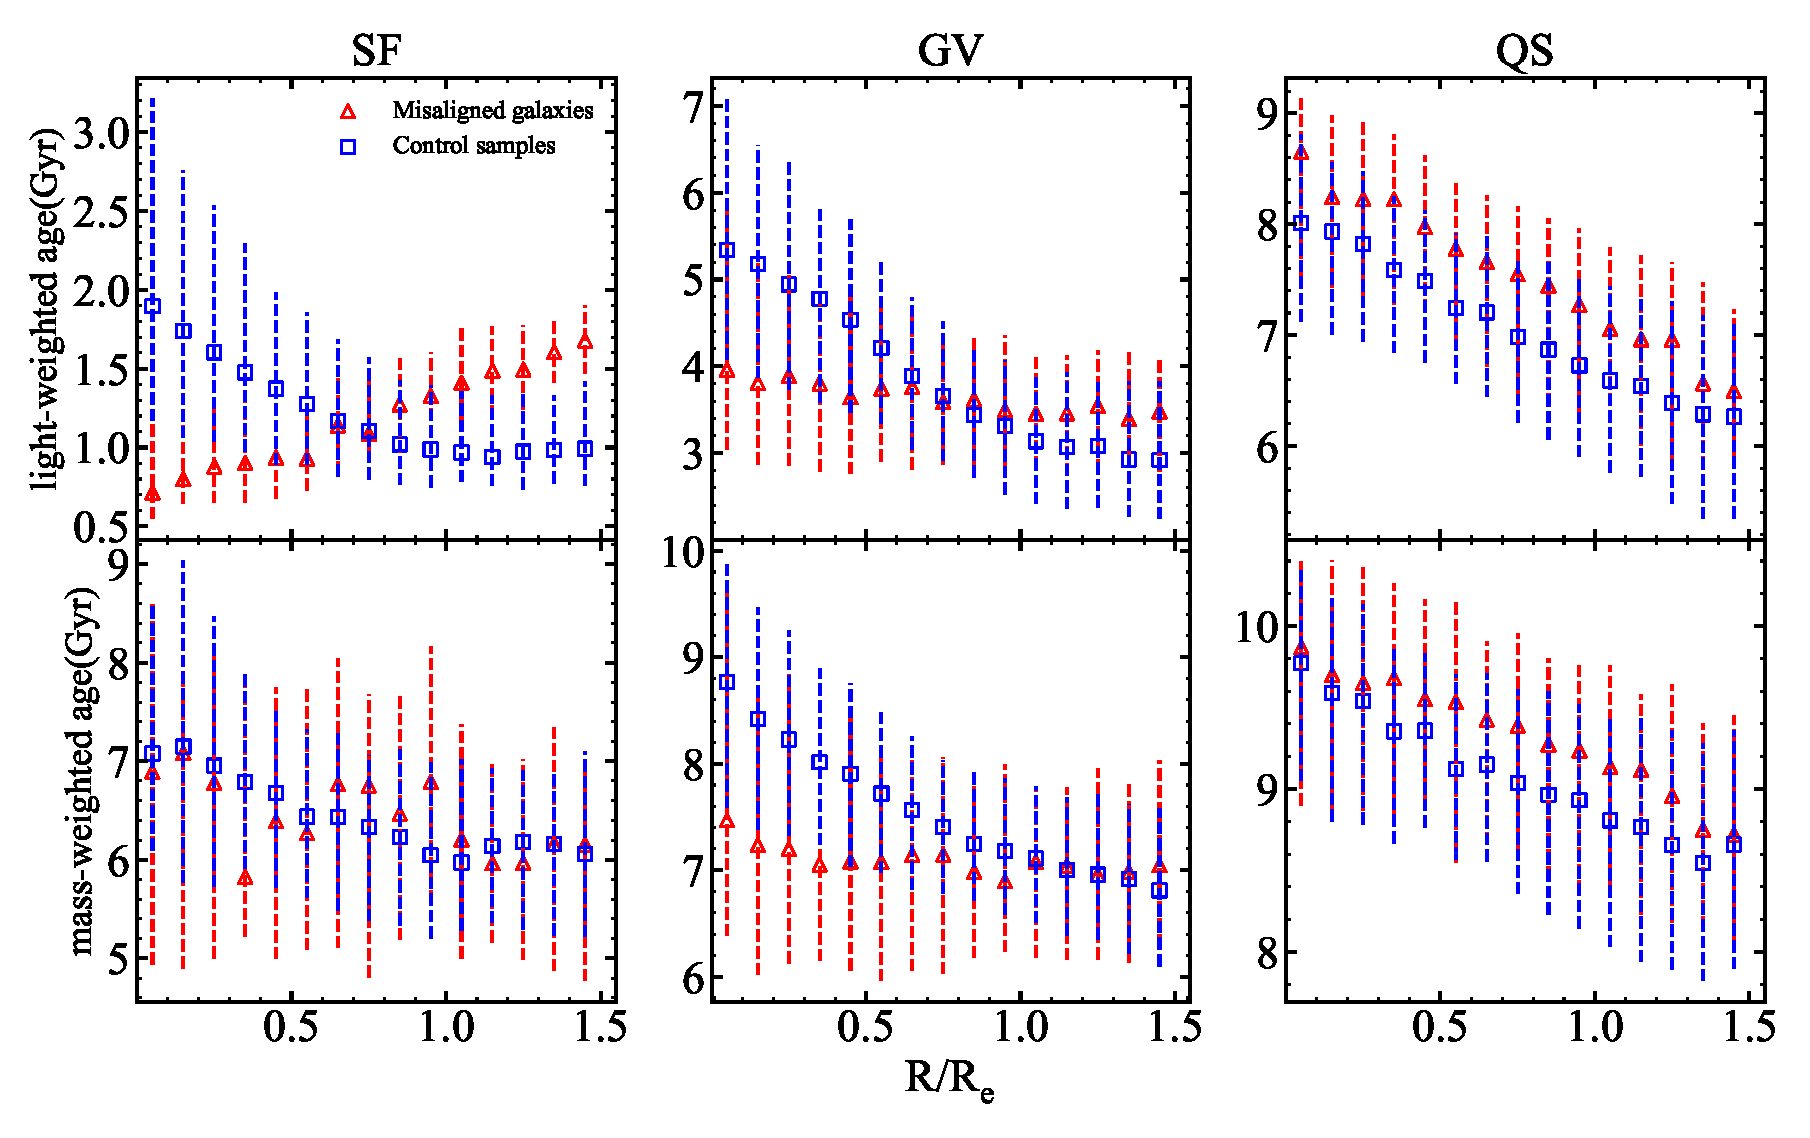
\includegraphics[width=2.0\columnwidth]{pics/lw_age_and_mw_age.eps}
    \caption{Comparison of light-weighted stellar ages and mass-weighted stellar age radial profiles within 1.5 $R_{\rm e}$ between misaligned galaxies and control sample. Red triangles represent misaligned galaxies and blue squares represent control sample.}
    \label{fig:lw_age_and_mw_age}
\end{figure*}

\begin{figure*}
    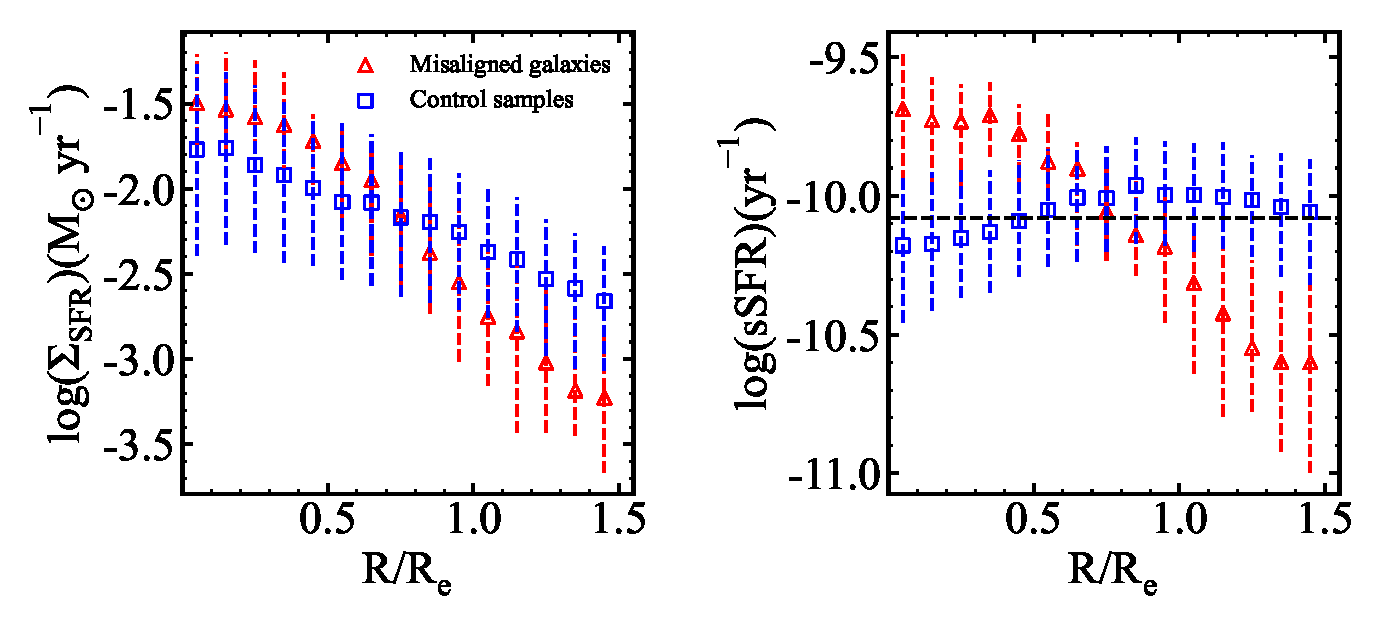
\includegraphics[width=1.6\columnwidth]{pics/SFR_and_sSFR.eps}
    \caption{Comparison of star formation rate surface density and specific star formation rate radial profiles within 1.5 $R_{\rm e}$ between SF misaligned galaxies and control sample. Red triangles represent misaligned galaxies and blue squares represent control sample. The horizontal dashed line is defined as 1/($t_{\rm{H}(z)}-1\,\rm Gyr$), where $t_{\rm{H}(z)}$ is the Hubble time at the median redshift of the MaNGA star forming galaxy sample.}
    \label{fig:SFR_and_sSFR}
\end{figure*}

\subsection{Stellar population}

In this section, we study the stellar population distribution of the misaligned galaxies and control sample using continuum spectral indices D$_n$4000, light-weighted stellar age and mass-weighted stellar age as well as the ongoing star formation rate. 

Fig.~\ref{fig:Dn(4000)} shows the D$_n$4000 radial profiles for the SF (left), GV (middle) and QS (right) galaxies. Again, red triangles represent misaligned galaxies and blue squares represent control sample. For the star-forming galaxies, the D$_n$4000 gradient of misaligned galaxies is positive while the gradient of control sample is negative. At $R$ < $\sim$0.7 $R_{\rm e}$, the median value of D$_n$4000 is lower (younger in stellar population) for the misaligned galaxies than the control sample. Over this radius, the result is totally inverse, the stellar population in misaligned galaxies becomes older (higher D$_n$4000) than the control galaxies. This is consistent with the results in \citet{chen_growth_2016}, \citet{jin_sdss-iv_2016} and \citet{bizyaev_sdss_2019}, indicating that SF misaligned galaxies have younger stellar population in the centre than that in the outskirts. The explanation for this outside-in growth mode in SF misaligned galaxies is that the redistribution of angular momentum occurs from gas-gas collisions between the pre-existing and the accreted gas largely accelerates gas inflow, on the one hand leading to a fast centrally concentrated star formation, on the other hand shutting down the star formation in the outskirts due to the lack of cold gas. The controls have a negative gradient in D$_n$4000, indicating older stellar populations in the centre, as expected for ordinary bulge+disk structure of star-forming galaxies, consistent with the inside-out growth mode. For the GV misaligned galaxies (middle panel), the median D$_n$4000 has a flat distribution over radius, with a roughly constant value of 1.7, while control sample has a negative gradient in D$_n$4000. Similar to the SF galaxies, the stellar population is younger with lower D$_n$4000 in the misaligned galaxies than the control sample at $R$ < $\sim$0.7 $R_{\rm e}$, and older over this radius. This suggests that the GV galaxies was undergoing similar process after external gas accretion as the SF galaxies. The smaller difference in D$_n$4000 between GV misaligned galaxies and the control sample indicates that this process happened either earlier or less violent than SF galaxies. The misaligned QS and their control galaxies have identical negative D$_n$4000 gradients, indicating external gas accretion either happened much earlier than the SF and GV galaxies or the influence on stellar population is negligible. The difference in D$_n$4000 between the misaligned galaxies and control sample decreases from SF to QS.

Fig.~\ref{fig:lw_age_and_mw_age} shows radial profiles in light-weighted stellar age (top row) and mass-weighted stellar age (bottom row). The two ages are taken from the Pipe3D Value Added Catalog \citep{2016RMxAA..52...21S, 2016RMxAA..52..171S}, in which the stellar continuum is fitted as a linear combination of synthetic single stellar population (SSP) templates. Again red triangles represent misaligned galaxies and blue squares represent the control sample. Since D$_n$4000 is a good indicator of light-weighted age of a stellar population, the radial profiles of light-weighted age and D$_n$4000 are very similar. It enhances the difference between misaligned galaxies and control sample, which can be seen from the distinct difference of light-weighted age in QS while D$_n$4000 shows little difference in QS. Mass-weighted ages of the SF misaligned galaxies show an overall flat distribution of old stellar population along radius (6$\sim$7 Gyr), which is totally different from the positive gradient of the light-weighted ages. Similar to the SF misaligned galaxies, the mass-weighted age gradient of their control sample is very shallow, and has similar value to that of misaligned galaxies. This suggests the underlying stellar population of the star forming misaligned galaxies is similar to the control samples, the current central concentrated star formation is simply a recent burst on top of a dominant old population. The misaligned galaxies in GV have a median mass-weighted age of 7$\sim$8 Gyr across the whole galaxies. At $R$ < 0.7$\sim$0.8 $R_{\rm e}$, it is $\sim$1 Gyr younger than the control samples (middle panel of Fig.~\ref{fig:lw_age_and_mw_age}) and becomes consistent with the controls at outskirts. For the misaligned QS galaxies, we find that their mass weighted ages are consistent with the control samples over radius, there is weak evidence that the misaligned galaxies are a little bit older, we do not tend to explain this tiny difference considering that the error bar of mass-weighted age measurement is quite large.

We estimate star formation rate surface density ($\Sigma_{\rm SFR}$) of star forming regions from the dust extinction corrected $\ha$ luminosity \citep{salpeter_luminosity_1955, kennicutt_star_1998} : $\rm SFR(M_{\sun} \ yr^{-1}) = 7.9 \times 10^{-42} \ L_{\ha} (erg \ s^{-1})$. Dust extinction is calculated from Balmer decrement ($\ha$ and $\hb$ flux ratio) under Case B, the Galactic dust extinction curve from \citet{calzetti_dust_2001} is applied. 
The specific star formation rate (sSFR) is defined as SFR/$M_*$ for each spaxel.

Fig.~\ref{fig:SFR_and_sSFR} shows radial profiles of the star formation rate surface density (left panel) and specific star formation rate (right panel) for SF galaxies. Again red triangles represent misaligned galaxies and blue squares represent the control samples. We only calculated $\Sigma_{\rm SFR}$ and sSFR for SF galaxies since there are very few star forming spaxels in GV and QS galaxies. As we can see, misaligned galaxies have higher $\Sigma_{\rm SFR}$ and sSFR within 0.7$\sim$0.8 $R_{\rm e}$ than their control sample, indicating that misaligned galaxies have enhanced recent star forming activity in the central regions. The horizontal dashed line in the right panel of Fig.~\ref{fig:SFR_and_sSFR} is defined as 1/($t_{\rm{H}(z)}-1\,\rm Gyr$), where $t_{\rm{H}(z)}$ is the Hubble time at the median redshift of the MaNGA star forming galaxy sample, and 1 Gyr is subtracted to account for the fact star formation primarily occurred after reionization. The higher sSFR for the central region of the misaligned sample than the value marked by the horizontal dashed line indicates that current SFR of the misaligned galaxies are higher than the past average ($M_*/(t_{\rm{H}(z)}-1\,\rm Gyr)$) of the local star forming galaxies, while the control sample have a current SFR which is similar to the past average, indicating fast growth of the central regions in the misaligned galaxies triggered by external gas accretion.

\subsection{Gas-phase metallicity}

\begin{figure*}
    
\includegraphics[width=2.0\columnwidth]{pics/metallicity.eps}
    \caption{Comparison of the radial profiles of gas-phase metallicities estimated from three different strong-line calibrators. Red triangles represent SF misaligned galaxies and blue squares represent the control samples. The left panel of Fig.~\ref{fig:metallicity} applies $R_{23}$ as the metallicity calibrator (Eq.1 in \citet{tremonti_origin_2004}), the middle panel applies O3N2 as the metallicity calibrator (Eq.2 in \citet{marino2013o3n2}), while N2S2\&N2$\ha$ is used in the right panel (Eq.2 in \citet{dopita_chemical_2016}). Red and blue crosses in left panel mark the median value of central $3^{\prime \prime}$ gas-phase metallicity from MPA-JHU catalogue for misaligned galaxies and control samples.}
    \label{fig:metallicity}
\end{figure*}

\begin{figure*}
    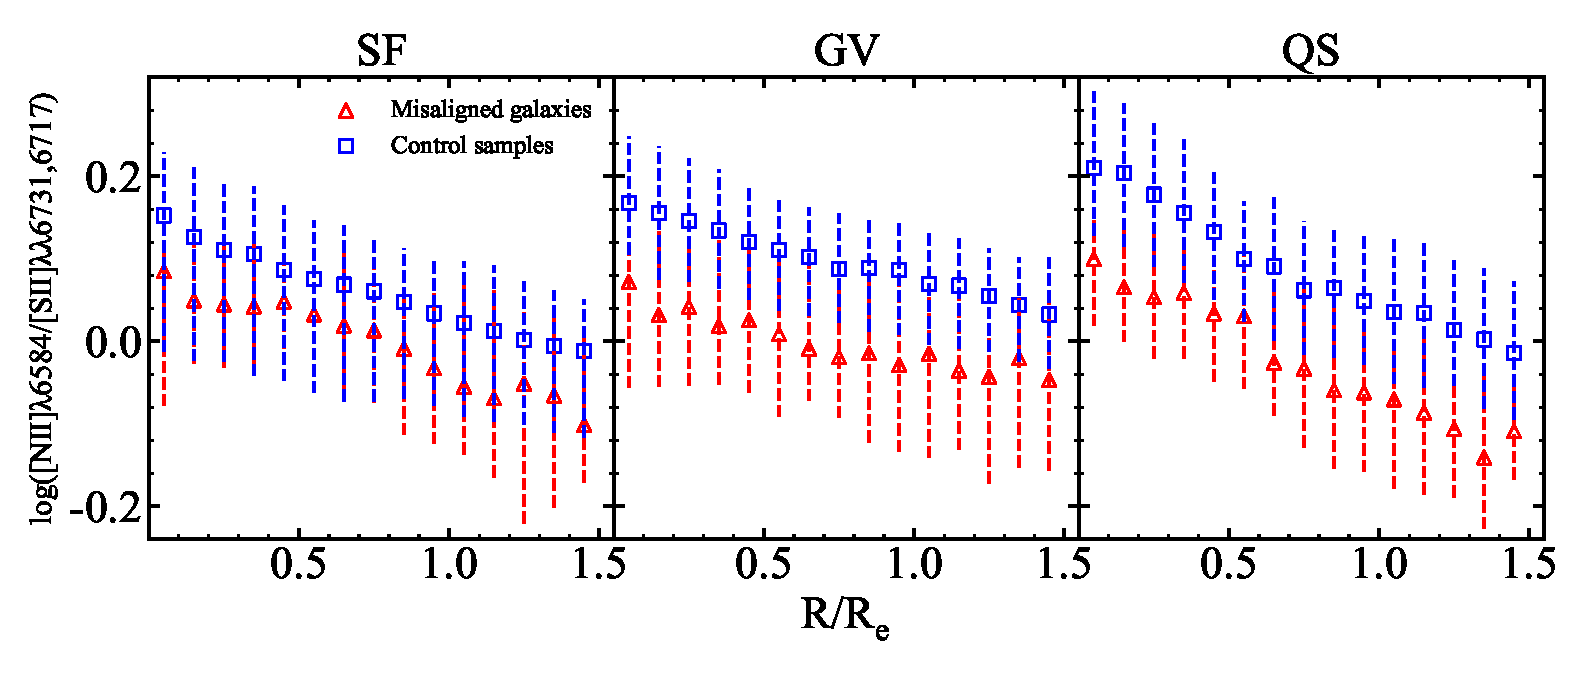
\includegraphics[width=2.0\columnwidth]{pics/NII_SII.eps}
    \caption{Comparison of {\nii}$\lambda$6584/{\sii}$\lambda\lambda$6717,6731 radial profiles within 1.5 $R_{\rm e}$ between misaligned galaxies and control sample. Red triangles represent misaligned galaxies and blue squares represent control sample.}
    \label{fig:NII_SII}
\end{figure*}

Gas-phase metallicity is one of the most fundamental physical properties of galaxies, it reflects the amount of gas reprocessed by stars and any exchange of gas between a galaxy and its environment.

The misaligned galaxies are believed to be the primary demonstrations whose evolution is regulated by external processes. External processes, such as minor/major mergers or gas accretion, could bring misaligned gas which has different metallicities from pre-existing gas into the galaxies. Thus, comparing the gas-phase metallicity between misaligned galaxies with their non-misaligned control sample will give us clues about the origin of misaligned gas as well as how the gas accretion processes influence the galaxy evolution.

Fig.~\ref{fig:metallicity} shows the radial profiles of gas-phase metallicity (estimated from three different strong line metallicity calibrators) for SF misaligned galaxies (red triangles) as well as their control samples (blue squares). The left panel of Fig.~\ref{fig:metallicity} applies $R_{23}$ as the metallicity calibrator (Eq.1 in \citet{tremonti_origin_2004}), the middle panel applies O3N2 as the metallicity calibrator (Eq.2 in \citet{marino2013o3n2}), while N2S2 and N2$\ha$ is used in the right panel (Eq.2 in \citet{dopita_chemical_2016}). Comparing the metallicities estimated from these three different calibrators, we find that although the absolute values and radial gradients of metallicity are different when we use different calibrators, they all point to the same conclusion that SF misaligned galaxies have overall lower gas-phase metallicity than their control samples. We do not discuss the difference in metallicities given by different calibrators in this work since unexpected systematic effect has been found by using different metallicity calibrators due to various reasons \citep{kewley_metallicity_2008, schaefer_sdss-iv_2019}.

Considering that the strong-line abundance diagnostics are developed based on the stellar population synthesis and photoionization models, it is limited to be only applied to $\hii$ regions \citep{kewley_using_2002}. However, the gas in the GV and QS galaxies is not excited by star formation for most of the spaxels, we thus follow \citet{jin_sdss-iv_2016} to apply $\nii\lambda6584/\sii\lambda\lambda6731,6717$ as an alternative gas-phase metallicity indicator. It is suggested by \citet{dopita_chemical_2016} and \citet{kashino2016hide} that $\nii\lambda6584/\sii\lambda\lambda6731,6717$ is a proxy for N/O ratio, and correlates with O/H abundance very well at 12 + log(O/H) $>$ 8.0. Also, the two emission lines are close in wavelength so the dust extinction correction is negligible. Fig.~\ref{fig:NII_SII} shows the radial gradients of $\nii\lambda6584/\sii\lambda\lambda6731,6717$ for the SF (left panel), GV (middle panel) and QS (right panel) misaligned galaxies (red triangles) as well as their control galaxies (blue squares). Similar to Fig.~\ref{fig:metallicity}, we find that the misaligned galaxies have lower gas-phase metallicities than their control samples, not only for the star forming galaxies, but also for green valley and quiescent galaxies, supporting the conclusion that the misaligned galaxies accreted low abundance gas from a gas-rich dwarf or cosmic web.

We have to point out that for the star forming misaligned galaxies, the difference in gas-phase metallicity between the misaligned galaxies and their controls strongly depends on how we define the control samples. We will discuss this in Section \ref{sec:discussion-1}.
